% Options for packages loaded elsewhere
\PassOptionsToPackage{unicode}{hyperref}
\PassOptionsToPackage{hyphens}{url}
\PassOptionsToPackage{dvipsnames,svgnames,x11names}{xcolor}
%
\documentclass[
  letterpaper,
  DIV=11,
  numbers=noendperiod]{scrartcl}

\usepackage{amsmath,amssymb}
\usepackage{iftex}
\ifPDFTeX
  \usepackage[T1]{fontenc}
  \usepackage[utf8]{inputenc}
  \usepackage{textcomp} % provide euro and other symbols
\else % if luatex or xetex
  \usepackage{unicode-math}
  \defaultfontfeatures{Scale=MatchLowercase}
  \defaultfontfeatures[\rmfamily]{Ligatures=TeX,Scale=1}
\fi
\usepackage{lmodern}
\ifPDFTeX\else  
    % xetex/luatex font selection
\fi
% Use upquote if available, for straight quotes in verbatim environments
\IfFileExists{upquote.sty}{\usepackage{upquote}}{}
\IfFileExists{microtype.sty}{% use microtype if available
  \usepackage[]{microtype}
  \UseMicrotypeSet[protrusion]{basicmath} % disable protrusion for tt fonts
}{}
\makeatletter
\@ifundefined{KOMAClassName}{% if non-KOMA class
  \IfFileExists{parskip.sty}{%
    \usepackage{parskip}
  }{% else
    \setlength{\parindent}{0pt}
    \setlength{\parskip}{6pt plus 2pt minus 1pt}}
}{% if KOMA class
  \KOMAoptions{parskip=half}}
\makeatother
\usepackage{xcolor}
\setlength{\emergencystretch}{3em} % prevent overfull lines
\setcounter{secnumdepth}{-\maxdimen} % remove section numbering
% Make \paragraph and \subparagraph free-standing
\ifx\paragraph\undefined\else
  \let\oldparagraph\paragraph
  \renewcommand{\paragraph}[1]{\oldparagraph{#1}\mbox{}}
\fi
\ifx\subparagraph\undefined\else
  \let\oldsubparagraph\subparagraph
  \renewcommand{\subparagraph}[1]{\oldsubparagraph{#1}\mbox{}}
\fi

\usepackage{color}
\usepackage{fancyvrb}
\newcommand{\VerbBar}{|}
\newcommand{\VERB}{\Verb[commandchars=\\\{\}]}
\DefineVerbatimEnvironment{Highlighting}{Verbatim}{commandchars=\\\{\}}
% Add ',fontsize=\small' for more characters per line
\usepackage{framed}
\definecolor{shadecolor}{RGB}{241,243,245}
\newenvironment{Shaded}{\begin{snugshade}}{\end{snugshade}}
\newcommand{\AlertTok}[1]{\textcolor[rgb]{0.68,0.00,0.00}{#1}}
\newcommand{\AnnotationTok}[1]{\textcolor[rgb]{0.37,0.37,0.37}{#1}}
\newcommand{\AttributeTok}[1]{\textcolor[rgb]{0.40,0.45,0.13}{#1}}
\newcommand{\BaseNTok}[1]{\textcolor[rgb]{0.68,0.00,0.00}{#1}}
\newcommand{\BuiltInTok}[1]{\textcolor[rgb]{0.00,0.23,0.31}{#1}}
\newcommand{\CharTok}[1]{\textcolor[rgb]{0.13,0.47,0.30}{#1}}
\newcommand{\CommentTok}[1]{\textcolor[rgb]{0.37,0.37,0.37}{#1}}
\newcommand{\CommentVarTok}[1]{\textcolor[rgb]{0.37,0.37,0.37}{\textit{#1}}}
\newcommand{\ConstantTok}[1]{\textcolor[rgb]{0.56,0.35,0.01}{#1}}
\newcommand{\ControlFlowTok}[1]{\textcolor[rgb]{0.00,0.23,0.31}{#1}}
\newcommand{\DataTypeTok}[1]{\textcolor[rgb]{0.68,0.00,0.00}{#1}}
\newcommand{\DecValTok}[1]{\textcolor[rgb]{0.68,0.00,0.00}{#1}}
\newcommand{\DocumentationTok}[1]{\textcolor[rgb]{0.37,0.37,0.37}{\textit{#1}}}
\newcommand{\ErrorTok}[1]{\textcolor[rgb]{0.68,0.00,0.00}{#1}}
\newcommand{\ExtensionTok}[1]{\textcolor[rgb]{0.00,0.23,0.31}{#1}}
\newcommand{\FloatTok}[1]{\textcolor[rgb]{0.68,0.00,0.00}{#1}}
\newcommand{\FunctionTok}[1]{\textcolor[rgb]{0.28,0.35,0.67}{#1}}
\newcommand{\ImportTok}[1]{\textcolor[rgb]{0.00,0.46,0.62}{#1}}
\newcommand{\InformationTok}[1]{\textcolor[rgb]{0.37,0.37,0.37}{#1}}
\newcommand{\KeywordTok}[1]{\textcolor[rgb]{0.00,0.23,0.31}{#1}}
\newcommand{\NormalTok}[1]{\textcolor[rgb]{0.00,0.23,0.31}{#1}}
\newcommand{\OperatorTok}[1]{\textcolor[rgb]{0.37,0.37,0.37}{#1}}
\newcommand{\OtherTok}[1]{\textcolor[rgb]{0.00,0.23,0.31}{#1}}
\newcommand{\PreprocessorTok}[1]{\textcolor[rgb]{0.68,0.00,0.00}{#1}}
\newcommand{\RegionMarkerTok}[1]{\textcolor[rgb]{0.00,0.23,0.31}{#1}}
\newcommand{\SpecialCharTok}[1]{\textcolor[rgb]{0.37,0.37,0.37}{#1}}
\newcommand{\SpecialStringTok}[1]{\textcolor[rgb]{0.13,0.47,0.30}{#1}}
\newcommand{\StringTok}[1]{\textcolor[rgb]{0.13,0.47,0.30}{#1}}
\newcommand{\VariableTok}[1]{\textcolor[rgb]{0.07,0.07,0.07}{#1}}
\newcommand{\VerbatimStringTok}[1]{\textcolor[rgb]{0.13,0.47,0.30}{#1}}
\newcommand{\WarningTok}[1]{\textcolor[rgb]{0.37,0.37,0.37}{\textit{#1}}}

\providecommand{\tightlist}{%
  \setlength{\itemsep}{0pt}\setlength{\parskip}{0pt}}\usepackage{longtable,booktabs,array}
\usepackage{calc} % for calculating minipage widths
% Correct order of tables after \paragraph or \subparagraph
\usepackage{etoolbox}
\makeatletter
\patchcmd\longtable{\par}{\if@noskipsec\mbox{}\fi\par}{}{}
\makeatother
% Allow footnotes in longtable head/foot
\IfFileExists{footnotehyper.sty}{\usepackage{footnotehyper}}{\usepackage{footnote}}
\makesavenoteenv{longtable}
\usepackage{graphicx}
\makeatletter
\def\maxwidth{\ifdim\Gin@nat@width>\linewidth\linewidth\else\Gin@nat@width\fi}
\def\maxheight{\ifdim\Gin@nat@height>\textheight\textheight\else\Gin@nat@height\fi}
\makeatother
% Scale images if necessary, so that they will not overflow the page
% margins by default, and it is still possible to overwrite the defaults
% using explicit options in \includegraphics[width, height, ...]{}
\setkeys{Gin}{width=\maxwidth,height=\maxheight,keepaspectratio}
% Set default figure placement to htbp
\makeatletter
\def\fps@figure{htbp}
\makeatother

\KOMAoption{captions}{tableheading}
\makeatletter
\makeatother
\makeatletter
\makeatother
\makeatletter
\@ifpackageloaded{caption}{}{\usepackage{caption}}
\AtBeginDocument{%
\ifdefined\contentsname
  \renewcommand*\contentsname{Table of contents}
\else
  \newcommand\contentsname{Table of contents}
\fi
\ifdefined\listfigurename
  \renewcommand*\listfigurename{List of Figures}
\else
  \newcommand\listfigurename{List of Figures}
\fi
\ifdefined\listtablename
  \renewcommand*\listtablename{List of Tables}
\else
  \newcommand\listtablename{List of Tables}
\fi
\ifdefined\figurename
  \renewcommand*\figurename{Figure}
\else
  \newcommand\figurename{Figure}
\fi
\ifdefined\tablename
  \renewcommand*\tablename{Table}
\else
  \newcommand\tablename{Table}
\fi
}
\@ifpackageloaded{float}{}{\usepackage{float}}
\floatstyle{ruled}
\@ifundefined{c@chapter}{\newfloat{codelisting}{h}{lop}}{\newfloat{codelisting}{h}{lop}[chapter]}
\floatname{codelisting}{Listing}
\newcommand*\listoflistings{\listof{codelisting}{List of Listings}}
\makeatother
\makeatletter
\@ifpackageloaded{caption}{}{\usepackage{caption}}
\@ifpackageloaded{subcaption}{}{\usepackage{subcaption}}
\makeatother
\makeatletter
\@ifpackageloaded{tcolorbox}{}{\usepackage[skins,breakable]{tcolorbox}}
\makeatother
\makeatletter
\@ifundefined{shadecolor}{\definecolor{shadecolor}{rgb}{.97, .97, .97}}
\makeatother
\makeatletter
\makeatother
\makeatletter
\makeatother
\ifLuaTeX
  \usepackage{selnolig}  % disable illegal ligatures
\fi
\IfFileExists{bookmark.sty}{\usepackage{bookmark}}{\usepackage{hyperref}}
\IfFileExists{xurl.sty}{\usepackage{xurl}}{} % add URL line breaks if available
\urlstyle{same} % disable monospaced font for URLs
\hypersetup{
  pdftitle={Inventing Life Insurance Experience Data},
  pdfauthor={Philip Adams},
  colorlinks=true,
  linkcolor={blue},
  filecolor={Maroon},
  citecolor={Blue},
  urlcolor={Blue},
  pdfcreator={LaTeX via pandoc}}

\title{Inventing Life Insurance Experience Data}
\author{Philip Adams}
\date{}

\begin{document}
\maketitle
\ifdefined\Shaded\renewenvironment{Shaded}{\begin{tcolorbox}[frame hidden, interior hidden, enhanced, sharp corners, breakable, borderline west={3pt}{0pt}{shadecolor}, boxrule=0pt]}{\end{tcolorbox}}\fi

\hypertarget{dabbling-in-the-dark-arts-for-clicks}{%
\section{Dabbling in the Dark Arts for
Clicks}\label{dabbling-in-the-dark-arts-for-clicks}}

Knowing how to create fake believable data is at once valuable and
suspicious. On the one hand, it shows a deep understanding of the
processes and nuances of the data you are simulating. On the other hand,
it shows an understanding for evil. For my own sake, I would like to
think that I am too honest for the latter. If I ever were to fake
results for a real situation, it probably means that I am suffering
mental illness and need to be committed.

But, life insurance datasets are impossible to find. So I will make one
up. Turns out, it isn't easy getting something believable off the
ground. Thus, the risk of inspiring another Billion Dollar Bubble movie
is low.

\hypertarget{approach}{%
\section{Approach}\label{approach}}

Here I use R. I will generate a census of lives including deaths and
lapse information. Many of the features of this data are based on my
experiences working with life insurance data over the years.

I have done this in Python for the sake of my own education and to
compare methods. I discuss the issues of using Python in my blog.

\hypertarget{preparation}{%
\subsection{Preparation}\label{preparation}}

\begin{Shaded}
\begin{Highlighting}[]
\FunctionTok{library}\NormalTok{(data.table)}
\FunctionTok{library}\NormalTok{(data.table)}
\FunctionTok{library}\NormalTok{(plyr)}
\FunctionTok{library}\NormalTok{(tidyverse)}
\FunctionTok{library}\NormalTok{(arrow)}
\FunctionTok{library}\NormalTok{(parallel)}
\FunctionTok{library}\NormalTok{(rvinecopulib)}
\FunctionTok{library}\NormalTok{(patchwork)}
\FunctionTok{library}\NormalTok{(GGally)}

\FunctionTok{RNGkind}\NormalTok{(}\StringTok{"L\textquotesingle{}Ecuyer{-}CMRG"}\NormalTok{)}



\NormalTok{sILECPath }\OtherTok{\textless{}{-}} \StringTok{"/workspace/Projects/ILEC/VBT/Data/ilecdata\_20240119"}
\NormalTok{nPolicyCensusSize }\OtherTok{\textless{}{-}} \DecValTok{2000000}
\NormalTok{arrIssueYearRange }\OtherTok{\textless{}{-}} \DecValTok{2041}\SpecialCharTok{:}\DecValTok{2054}

\FunctionTok{set.seed}\NormalTok{(}\DecValTok{0xBEEF}\NormalTok{)}

\CommentTok{\# Low Face is 90\% of these, Males are 120\% of these}
\NormalTok{fLowFaceFactorTrue }\OtherTok{\textless{}{-}} \FloatTok{0.9}
\NormalTok{fMaleFactorTrue }\OtherTok{\textless{}{-}} \FloatTok{1.2}
\end{Highlighting}
\end{Shaded}

\hypertarget{building-a-source-distribution}{%
\subsection{Building a Source
Distribution}\label{building-a-source-distribution}}

I build a source distribution based on the ILEC data from 2011-2017.
This uses the distribution of risks for term business in duration 1
issued under a four-class preferred system, by issue age, sex, and face
amount. I weight by policies exposed. To expand by issue year, I create
a fake issue year table covering our futuristic issue year along with
relative proportion by issue year. The relative proportion is used to
weight the policies exposed from the prior step. This is meant to
simulate sales growth.

\begin{Shaded}
\begin{Highlighting}[]
\NormalTok{ilec\_dataset }\OtherTok{\textless{}{-}}\NormalTok{ arrow}\SpecialCharTok{::}\FunctionTok{open\_dataset}\NormalTok{(}
  \AttributeTok{sources=}\NormalTok{sILECPath,}
  \AttributeTok{format=}\StringTok{"parquet"}
\NormalTok{)}

\CommentTok{\# Extract the data}
\NormalTok{ilec\_dataset }\SpecialCharTok{\%\textgreater{}\%}
  \FunctionTok{filter}\NormalTok{(Insurance\_Plan }\SpecialCharTok{==} \StringTok{"Term"} \SpecialCharTok{\&}
\NormalTok{           Duration }\SpecialCharTok{==} \DecValTok{1} \SpecialCharTok{\&}
\NormalTok{           Issue\_Age }\SpecialCharTok{\textgreater{}=} \DecValTok{18} \SpecialCharTok{\&}
\NormalTok{           Issue\_Age }\SpecialCharTok{\textless{}=} \DecValTok{70} \SpecialCharTok{\&}
\NormalTok{           Number\_of\_Pfd\_Classes }\SpecialCharTok{==} \StringTok{"4"} \SpecialCharTok{\&}
\NormalTok{           Observation\_Year }\SpecialCharTok{\textgreater{}=} \DecValTok{2011} \SpecialCharTok{\&}
\NormalTok{           Observation\_Year }\SpecialCharTok{\textless{}=} \DecValTok{2017}\NormalTok{) }\SpecialCharTok{\%\textgreater{}\%}
  \FunctionTok{group\_by}\NormalTok{(Sex,Issue\_Age,Face\_Amount\_Band) }\SpecialCharTok{\%\textgreater{}\%}
  \FunctionTok{summarize}\NormalTok{(}\AttributeTok{Policies\_Exposed=}\FunctionTok{sum}\NormalTok{(Policies\_Exposed)) }\SpecialCharTok{\%\textgreater{}\%}
  \FunctionTok{collect}\NormalTok{() }\SpecialCharTok{\%\textgreater{}\%}
  \FunctionTok{data.table}\NormalTok{() }\OtherTok{{-}\textgreater{}}
\NormalTok{  src\_distribution}

\CommentTok{\# Regroup the face amounts to low and high face}
\NormalTok{src\_distribution }\SpecialCharTok{\%\textgreater{}\%}
  \FunctionTok{mutate}\NormalTok{(}\AttributeTok{Face\_Group=}\FunctionTok{fct\_collapse}\NormalTok{(Face\_Amount\_Band,}
                                 \AttributeTok{Low\_Face=}\FunctionTok{c}\NormalTok{(}\StringTok{"01: 0 {-} 9,999"}\NormalTok{,}
                                            \StringTok{"02: 10,000 {-} 24,999"}\NormalTok{,}
                                            \StringTok{"03: 25,000 {-} 49,999"}\NormalTok{,}
                                            \StringTok{"04: 50,000 {-} 99,999"}\NormalTok{,}
                                            \StringTok{"05: 100,000 {-} 249,999"}\NormalTok{,}
                                            \StringTok{"06: 250,000 {-} 499,999"}\NormalTok{),}
                                 \AttributeTok{other\_level=}\StringTok{"High\_Face"}\NormalTok{)}
\NormalTok{  ) }\SpecialCharTok{\%\textgreater{}\%}
  \FunctionTok{group\_by}\NormalTok{(Sex,Issue\_Age,Face\_Group) }\SpecialCharTok{\%\textgreater{}\%}
  \FunctionTok{summarize}\NormalTok{(}\AttributeTok{Policies\_Exposed=}\FunctionTok{sum}\NormalTok{(Policies\_Exposed)) }\SpecialCharTok{\%\textgreater{}\%}
  \FunctionTok{arrange}\NormalTok{(Sex,Issue\_Age,Face\_Group) }\SpecialCharTok{\%\textgreater{}\%}
  \FunctionTok{data.table}\NormalTok{() }\OtherTok{{-}\textgreater{}}
\NormalTok{  src\_distribution}

\CommentTok{\# Expand the issue year dimension and adjust the exposure per year}
\NormalTok{src\_distribution }\SpecialCharTok{\%\textgreater{}\%}
  \FunctionTok{cross\_join}\NormalTok{(}
    \FunctionTok{data.table}\NormalTok{( }\AttributeTok{Issue\_Year=}\NormalTok{arrIssueYearRange,}
                \AttributeTok{Proportion=}\FunctionTok{seq}\NormalTok{(.}\DecValTok{8}\NormalTok{,}\FloatTok{1.3}\NormalTok{,}\AttributeTok{length=}\FunctionTok{length}\NormalTok{(arrIssueYearRange)))}
\NormalTok{  ) }\SpecialCharTok{\%\textgreater{}\%}
  \FunctionTok{mutate}\NormalTok{(}\AttributeTok{Policies\_Exposed=}\NormalTok{Policies\_Exposed}\SpecialCharTok{*}\NormalTok{Proportion) }\SpecialCharTok{\%\textgreater{}\%}
  \FunctionTok{select}\NormalTok{(}\SpecialCharTok{{-}}\NormalTok{Proportion) }\OtherTok{{-}\textgreater{}}
\NormalTok{  src\_distribution}

\FunctionTok{head}\NormalTok{(src\_distribution)}
\end{Highlighting}
\end{Shaded}

\begin{verbatim}
      Sex Issue_Age Face_Group Policies_Exposed Issue_Year
   <char>     <int>     <fctr>            <num>      <int>
1:      F        18   Low_Face         1662.965       2041
2:      F        18   Low_Face         1742.915       2042
3:      F        18   Low_Face         1822.865       2043
4:      F        18   Low_Face         1902.815       2044
5:      F        18   Low_Face         1982.766       2045
6:      F        18   Low_Face         2062.716       2046
\end{verbatim}

\hypertarget{building-a-policy-census}{%
\subsection{Building a Policy Census}\label{building-a-policy-census}}

To sample a census, I randomly sample rows from the source distribution
table. Then I construct random issue dates within a calendar year. While
the day of the month is random, the month is weighted toward the end of
the year and away from the beginning of the year. Many companies will
create sales incentives that increase sales at the end of the year,
often at the expense of sales in the first quarter.

\begin{Shaded}
\begin{Highlighting}[]
\CommentTok{\# Sample the source distribution to build a policy listing}
\NormalTok{policy\_pop }\OtherTok{\textless{}{-}}\NormalTok{ src\_distribution[}
  \FunctionTok{sample.int}\NormalTok{(}\AttributeTok{n=}\FunctionTok{nrow}\NormalTok{(src\_distribution),}
             \AttributeTok{size=}\NormalTok{nPolicyCensusSize,}
             \AttributeTok{replace=}\NormalTok{T,}
             \AttributeTok{prob=}\NormalTok{src\_distribution}\SpecialCharTok{$}\NormalTok{Policies\_Exposed),}
\NormalTok{  .(Sex,Issue\_Age,Face\_Group,Issue\_Year)}
\NormalTok{]}

\CommentTok{\# Set an ID}
\NormalTok{policy\_pop[,PolID}\SpecialCharTok{:}\ErrorTok{=}\DecValTok{1}\SpecialCharTok{:}\FunctionTok{nrow}\NormalTok{(.SD)]}

\CommentTok{\# Issue Date}
\CommentTok{\# Create a table of months and days in a standard year, and then add a proportion}
\FunctionTok{data.table}\NormalTok{(}\AttributeTok{DayOfYear=}\DecValTok{1}\SpecialCharTok{:}\DecValTok{365}\NormalTok{) }\SpecialCharTok{\%\textgreater{}\%}
  \FunctionTok{mutate}\NormalTok{(}\AttributeTok{DateTemp =} \FunctionTok{ymd}\NormalTok{(}\DecValTok{20101231}\NormalTok{) }\SpecialCharTok{\%m+\%} \FunctionTok{days}\NormalTok{(DayOfYear),}
         \AttributeTok{Month=}\FunctionTok{month}\NormalTok{(DateTemp),}
         \AttributeTok{Day=}\FunctionTok{day}\NormalTok{(DateTemp),}
         \AttributeTok{Proportion=}\DecValTok{1}\SpecialCharTok{/}\DecValTok{365}\NormalTok{) }\SpecialCharTok{\%\textgreater{}\%}
  \FunctionTok{select}\NormalTok{(Month,Day,Proportion) }\OtherTok{{-}\textgreater{}} 
\NormalTok{  issue\_days}

\NormalTok{issue\_days[Month}\SpecialCharTok{==}\DecValTok{1}\NormalTok{,Proportion}\SpecialCharTok{:}\ErrorTok{=}\NormalTok{Proportion}\SpecialCharTok{*}\NormalTok{.}\DecValTok{5}\NormalTok{]}
\NormalTok{issue\_days[Month}\SpecialCharTok{==}\DecValTok{2}\NormalTok{,Proportion}\SpecialCharTok{:}\ErrorTok{=}\NormalTok{Proportion}\SpecialCharTok{/}\NormalTok{.}\DecValTok{7}\NormalTok{]}
\NormalTok{issue\_days[Month}\SpecialCharTok{==}\DecValTok{11}\NormalTok{,Proportion}\SpecialCharTok{:}\ErrorTok{=}\NormalTok{Proportion}\SpecialCharTok{/}\NormalTok{.}\DecValTok{7}\NormalTok{]}
\NormalTok{issue\_days[Month}\SpecialCharTok{==}\DecValTok{12}\NormalTok{,Proportion}\SpecialCharTok{:}\ErrorTok{=}\NormalTok{Proportion}\SpecialCharTok{/}\NormalTok{.}\DecValTok{5}\NormalTok{]}

\CommentTok{\# Sample a random day}
\NormalTok{policy\_pop }\OtherTok{\textless{}{-}} \FunctionTok{cbind}\NormalTok{(policy\_pop,}
\NormalTok{                          issue\_days[}
                            \FunctionTok{sample.int}\NormalTok{(}\AttributeTok{n=}\FunctionTok{nrow}\NormalTok{(issue\_days), }
                                       \AttributeTok{size=}\NormalTok{nPolicyCensusSize,}
                                       \AttributeTok{replace=}\NormalTok{T,}
                                       \AttributeTok{prob=}\NormalTok{issue\_days}\SpecialCharTok{$}\NormalTok{Proportion),}
\NormalTok{                            .(Month,Day)}
\NormalTok{                          ]}
\NormalTok{)}

\CommentTok{\# ... and create the issue date}
\NormalTok{policy\_pop }\SpecialCharTok{\%\textgreater{}\%}
  \FunctionTok{mutate}\NormalTok{(}\AttributeTok{Issue\_Date=}\FunctionTok{ymd}\NormalTok{(}\FunctionTok{paste0}\NormalTok{(Issue\_Year,}\StringTok{" "}\NormalTok{,Month,}\StringTok{" "}\NormalTok{,Day))) }\SpecialCharTok{\%\textgreater{}\%}
  \FunctionTok{select}\NormalTok{(}\SpecialCharTok{{-}}\NormalTok{Month,}\SpecialCharTok{{-}}\NormalTok{Day) }\OtherTok{{-}\textgreater{}}
\NormalTok{  policy\_pop}

\CommentTok{\# Face Amounts}
\CommentTok{\# Low face is 100{-}450K spaced at 50K intervals}
\CommentTok{\# High Face is 500K {-} 2M spaced at 100K intervals}
\NormalTok{policy\_pop[Face\_Group}\SpecialCharTok{==}\StringTok{"Low\_Face"}\NormalTok{,}
\NormalTok{           Face\_Amount}\SpecialCharTok{:}\ErrorTok{=}\DecValTok{1000}\SpecialCharTok{*}\FunctionTok{sample}\NormalTok{(}\AttributeTok{x=}\FunctionTok{seq}\NormalTok{(}\DecValTok{100}\NormalTok{,}\DecValTok{450}\NormalTok{,}\DecValTok{50}\NormalTok{),}
                               \AttributeTok{size=}\FunctionTok{nrow}\NormalTok{(.SD),}
                               \AttributeTok{replace=}\NormalTok{T)}
\NormalTok{]}

\NormalTok{policy\_pop[Face\_Group}\SpecialCharTok{==}\StringTok{"High\_Face"}\NormalTok{,}
\NormalTok{           Face\_Amount}\SpecialCharTok{:}\ErrorTok{=}\DecValTok{1000}\SpecialCharTok{*}\FunctionTok{sample}\NormalTok{(}\AttributeTok{x=}\FunctionTok{seq}\NormalTok{(}\DecValTok{500}\NormalTok{,}\DecValTok{2000}\NormalTok{,}\DecValTok{100}\NormalTok{),}
                                    \AttributeTok{size=}\FunctionTok{nrow}\NormalTok{(.SD),}
                                    \AttributeTok{replace=}\NormalTok{T)}
\NormalTok{]}

\CommentTok{\# Set a premium mode based on reasonable real world proportions}
\NormalTok{policy\_pop[,prem\_mode}\SpecialCharTok{:}\ErrorTok{=} \FunctionTok{sample}\NormalTok{(}\FunctionTok{c}\NormalTok{(}\StringTok{"A"}\NormalTok{,}\StringTok{"Q"}\NormalTok{,}\StringTok{"M"}\NormalTok{),}
                               \AttributeTok{size=}\FunctionTok{nrow}\NormalTok{(.SD),}
                               \AttributeTok{prob=}\FunctionTok{c}\NormalTok{(.}\DecValTok{04}\NormalTok{,.}\DecValTok{01}\NormalTok{,.}\DecValTok{95}\NormalTok{),}
                               \AttributeTok{replace=}\NormalTok{T)]}

\FunctionTok{head}\NormalTok{(policy\_pop)}
\end{Highlighting}
\end{Shaded}

\begin{verbatim}
      Sex Issue_Age Face_Group Issue_Year PolID Issue_Date Face_Amount
   <char>     <int>     <fctr>      <int> <int>     <Date>       <num>
1:      F        37   Low_Face       2054     1 2054-08-28      200000
2:      M        34   Low_Face       2049     2 2049-03-24      100000
3:      F        38   Low_Face       2052     3 2052-02-16      100000
4:      M        34  High_Face       2052     4 2052-09-22     1700000
5:      M        47  High_Face       2043     5 2043-10-18      900000
6:      M        62   Low_Face       2043     6 2043-11-14      300000
   prem_mode
      <char>
1:         M
2:         M
3:         M
4:         M
5:         M
6:         M
\end{verbatim}

\hypertarget{simulate-preferred-attributes-using-vine-copulas}{%
\subsection{Simulate Preferred Attributes Using Vine
Copulas}\label{simulate-preferred-attributes-using-vine-copulas}}

To simulate a believable distribution of preferred criteria, I use vine
copulas. The associated blog post explains these at a high level. Here,
we model Bot Mass Index (BMI), Oil Pressure, and Oil Viscosity using a
copula where BMI is dependent on each of oil pressure and oil viscosity,
and pressure and viscosity are dependent given BMI. The analogy to Body
Mass Index, blood pressure, and cholesterol might be coincidental.

The dependence of BMI to the others is a BB7 copula with parameters 1.5
and 3. The dependence of oil pressure and viscosity given BMI is
Gaussian with correlatio 0.4.

\begin{Shaded}
\begin{Highlighting}[]
\CommentTok{\# Create synthetic preferred distributions}
\CommentTok{\# BMI, oil pressure, and oil viscosity are modeled with a copula, which is }
\CommentTok{\# necessarily a cvine (3 variables)}
\NormalTok{pref.vine }\OtherTok{\textless{}{-}} \FunctionTok{vinecop\_dist}\NormalTok{(}
  \AttributeTok{pair\_copulas =} \FunctionTok{list}\NormalTok{(}
    \FunctionTok{list}\NormalTok{(}
      \FunctionTok{bicop\_dist}\NormalTok{(}\StringTok{"bb7"}\NormalTok{,}\DecValTok{180}\NormalTok{,}\FunctionTok{c}\NormalTok{(}\FloatTok{1.5}\NormalTok{,}\DecValTok{3}\NormalTok{)),}
      \FunctionTok{bicop\_dist}\NormalTok{(}\StringTok{"bb7"}\NormalTok{,}\DecValTok{180}\NormalTok{,}\FunctionTok{c}\NormalTok{(}\FloatTok{1.5}\NormalTok{,}\DecValTok{3}\NormalTok{))}
\NormalTok{    ),}
    \FunctionTok{list}\NormalTok{(}\FunctionTok{bicop\_dist}\NormalTok{(}\StringTok{"gaussian"}\NormalTok{,}\DecValTok{0}\NormalTok{,.}\DecValTok{4}\NormalTok{))}
\NormalTok{  ),}
  \AttributeTok{structure =} \FunctionTok{cvine\_structure}\NormalTok{(}\DecValTok{1}\SpecialCharTok{:}\DecValTok{3}\NormalTok{)}
\NormalTok{)}

\NormalTok{pref.vine}\SpecialCharTok{$}\NormalTok{names }\OtherTok{\textless{}{-}} \FunctionTok{c}\NormalTok{(}\StringTok{"OilPressure"}\NormalTok{,}\StringTok{"OilViscosity"}\NormalTok{,}\StringTok{"BMI"}\NormalTok{)}

\CommentTok{\# Simulate the collectino of dependent uniform random variates}
\FunctionTok{rvinecop}\NormalTok{(}\AttributeTok{n=}\NormalTok{nPolicyCensusSize,}
\NormalTok{         pref.vine,}
         \AttributeTok{cores=}\DecValTok{8}\NormalTok{) }\OtherTok{{-}\textgreater{}}
\NormalTok{  pref.samples}

\NormalTok{pref.samples }\SpecialCharTok{\%\textgreater{}\%}
  \FunctionTok{as.data.table}\NormalTok{() }\SpecialCharTok{\%\textgreater{}\%}
  \FunctionTok{rename}\NormalTok{(}
    \AttributeTok{BMI\_u=}\NormalTok{BMI,}
    \AttributeTok{OilViscosity\_u=}\NormalTok{OilViscosity,}
    \AttributeTok{OilPressure\_u=}\NormalTok{OilPressure}
\NormalTok{  ) }\OtherTok{{-}\textgreater{}}\NormalTok{ pref.samples}

\NormalTok{policy\_pop }\SpecialCharTok{\%\textgreater{}\%}
  \FunctionTok{cbind}\NormalTok{(pref.samples) }\OtherTok{{-}\textgreater{}}
\NormalTok{  policy\_pop}
\end{Highlighting}
\end{Shaded}

It helps to visualize the vine and its distributions, and they can be
plotted.

\hypertarget{dependency-structure}{%
\subsubsection{Dependency Structure}\label{dependency-structure}}

\begin{Shaded}
\begin{Highlighting}[]
\FunctionTok{plot}\NormalTok{(pref.vine,}\AttributeTok{tree=}\DecValTok{1}\SpecialCharTok{:}\DecValTok{2}\NormalTok{, }\AttributeTok{edge\_labels =} \StringTok{"family\_tau"}\NormalTok{,}\AttributeTok{var\_names =} \StringTok{"legend"}\NormalTok{)}
\end{Highlighting}
\end{Shaded}

\begin{figure}[H]

{\centering 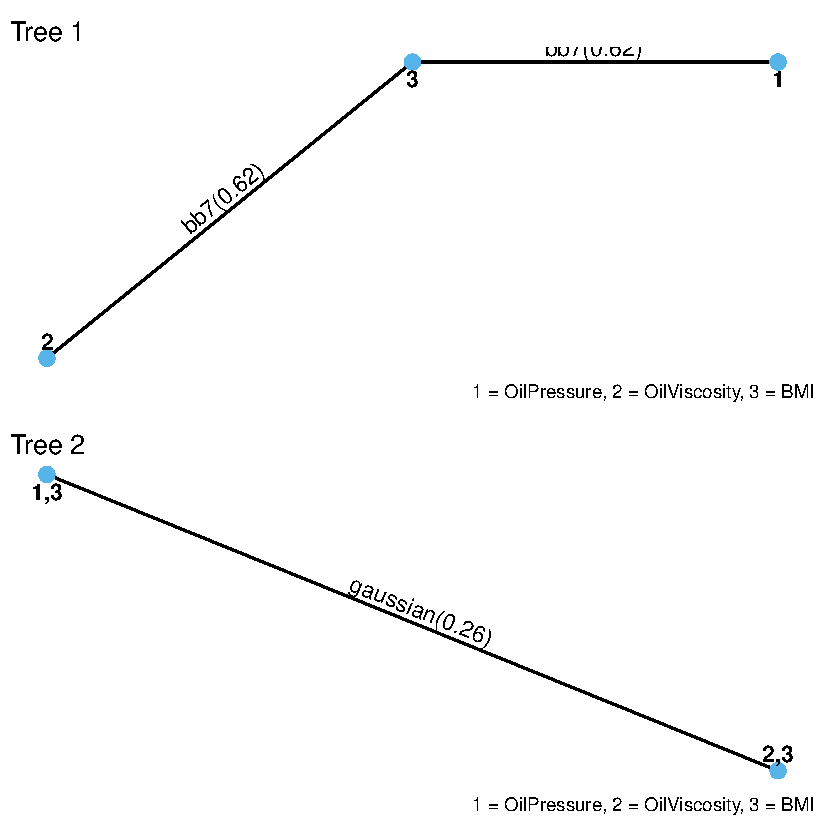
\includegraphics{MakingData_files/figure-pdf/unnamed-chunk-5-1.pdf}

}

\end{figure}

\hypertarget{contour-plots-of-bivariate-copulas}{%
\subsubsection{Contour plots of bivariate
copulas}\label{contour-plots-of-bivariate-copulas}}

It is easy to see here the strong upper tail dependence. The second
level has some correlation, but the expectation is that most of the
dependence will arise from BMI. Note that the Gaussian has no tail
dependence. Also note that the contour plots assume normal margins.

\begin{Shaded}
\begin{Highlighting}[]
\FunctionTok{contour}\NormalTok{(pref.vine)}
\end{Highlighting}
\end{Shaded}

\begin{figure}[H]

{\centering 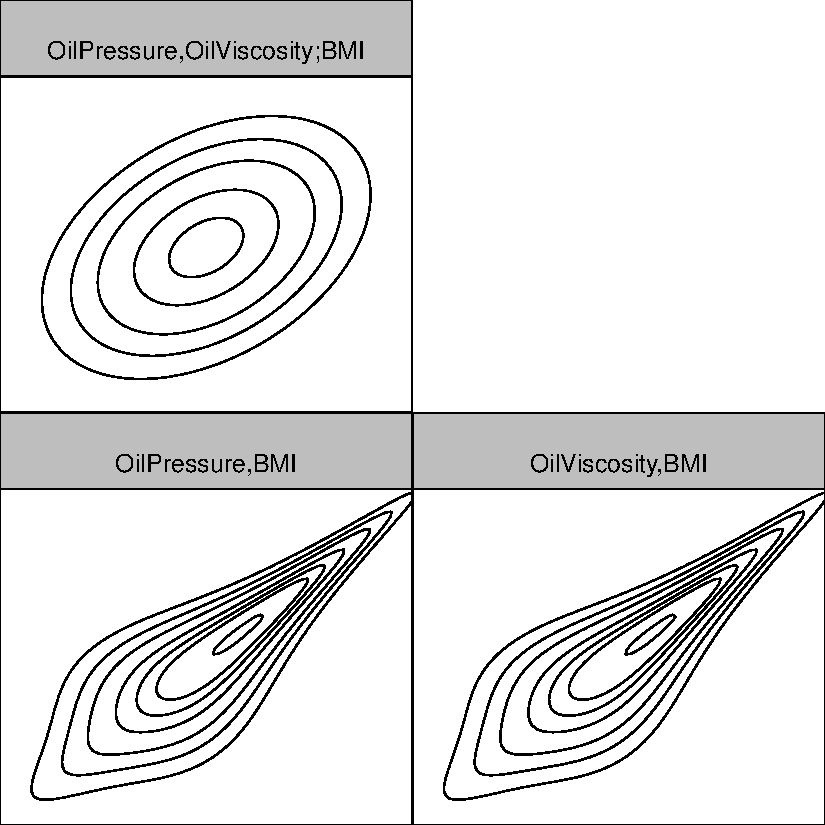
\includegraphics{MakingData_files/figure-pdf/unnamed-chunk-6-1.pdf}

}

\end{figure}

\hypertarget{convert-simulated-uniform-marginals-to-native-distribution}{%
\subsection{Convert Simulated Uniform Marginals to Native
Distribution}\label{convert-simulated-uniform-marginals-to-native-distribution}}

The simulator function for the vine copula generates values with uniform
margins, so they are converted to the distributional scale we need.

\begin{itemize}
\tightlist
\item
  Each margin uses a gamma distribution.
\item
  BMI for high face policies initially has mean 25 and variance 50.
\item
  Oil pressure for high face policies initially has mean 30 and variance
  20.
\item
  Oil viscosity for high face policies initially has mean 20 and
  variance 20.
\item
  Low face policies have mean 90\% of high face, and males have mean
  120\% over females (at 100\%).
\item
  Starting in 2046, the means increase by 1\% per issue year.
\end{itemize}

\begin{Shaded}
\begin{Highlighting}[]
\CommentTok{\# High Face}
\CommentTok{\# BMI is gamma with mean 25 and variance 50}
\CommentTok{\# Oil Pressure is gamma with mean 30 and variance 20}
\CommentTok{\# Oil viscosity is gamma with mean 20 and variance 20}

\CommentTok{\# Low Face is 90\% of these, Males are 120\% of these}
\CommentTok{\# Starting in year 2046, apply 1\% per issue year increase to all means}
\NormalTok{low\_face\_factor\_true }\OtherTok{\textless{}{-}} \FloatTok{0.9}
\NormalTok{male\_factor\_true }\OtherTok{\textless{}{-}} \FloatTok{1.2}

\CommentTok{\# Essentiall the inverse of the gamma CDF, but since we are specifying }
\CommentTok{\# everything using the mean and variance, these have to be translated }
\CommentTok{\# to shape and scale}
\NormalTok{convert\_marginal\_to\_gamma }\OtherTok{\textless{}{-}} \ControlFlowTok{function}\NormalTok{(x, }\AttributeTok{mean=}\DecValTok{1}\NormalTok{, }\AttributeTok{variance=}\DecValTok{1}\NormalTok{, }\AttributeTok{rounding=}\DecValTok{2}\NormalTok{) \{}
\NormalTok{  shape }\OtherTok{\textless{}{-}}\NormalTok{ mean}\SpecialCharTok{*}\NormalTok{mean}\SpecialCharTok{/}\NormalTok{variance}
\NormalTok{  scale }\OtherTok{\textless{}{-}}\NormalTok{ variance}\SpecialCharTok{/}\NormalTok{mean}
  
  \FunctionTok{round}\NormalTok{(}\FunctionTok{qgamma}\NormalTok{(x,}\AttributeTok{shape=}\NormalTok{shape,}\AttributeTok{scale=}\NormalTok{scale),rounding)}
\NormalTok{\}}

\NormalTok{policy\_pop[,PrefMeanFactor}\SpecialCharTok{:}\ErrorTok{=}\FunctionTok{ifelse}\NormalTok{(Sex}\SpecialCharTok{==}\StringTok{"Male"}\NormalTok{,male\_factor\_true,}\DecValTok{1}\NormalTok{)}\SpecialCharTok{*}
             \FunctionTok{ifelse}\NormalTok{(Face\_Group}\SpecialCharTok{==}\StringTok{"Low\_Face"}\NormalTok{,low\_face\_factor\_true,}\DecValTok{1}\NormalTok{)}\SpecialCharTok{*}
\NormalTok{             (}\DecValTok{1}\SpecialCharTok{+}\FunctionTok{pmax}\NormalTok{(}\DecValTok{0}\NormalTok{,Issue\_Year}\DecValTok{{-}2045}\NormalTok{)}\SpecialCharTok{/}\DecValTok{100}\NormalTok{)]}

\NormalTok{policy\_pop[,}
           \StringTok{\textasciigrave{}}\AttributeTok{:=}\StringTok{\textasciigrave{}}\NormalTok{(}
             \AttributeTok{BMI=}\FunctionTok{mapply}\NormalTok{(}\AttributeTok{FUN=}\NormalTok{convert\_marginal\_to\_gamma,}
\NormalTok{                        BMI\_u,}
                        \DecValTok{25}\SpecialCharTok{*}\NormalTok{PrefMeanFactor,}
                        \AttributeTok{variance=}\DecValTok{50}\NormalTok{),}
             \AttributeTok{OilPressure=}\FunctionTok{mapply}\NormalTok{(}\AttributeTok{FUN=}\NormalTok{convert\_marginal\_to\_gamma,}
\NormalTok{                                OilPressure\_u,}
                                \DecValTok{30}\SpecialCharTok{*}\NormalTok{PrefMeanFactor,}
                                \AttributeTok{variance=}\DecValTok{20}\NormalTok{),}
             \AttributeTok{OilViscosity=}\FunctionTok{mapply}\NormalTok{(}\AttributeTok{FUN=}\NormalTok{convert\_marginal\_to\_gamma,}
\NormalTok{                                OilViscosity\_u,}
                                \DecValTok{20}\SpecialCharTok{*}\NormalTok{PrefMeanFactor,}
                                \AttributeTok{variance=}\DecValTok{20}\NormalTok{)}
\NormalTok{           )]}


\NormalTok{policy\_pop[,}\StringTok{\textasciigrave{}}\AttributeTok{:=}\StringTok{\textasciigrave{}}\NormalTok{(}\AttributeTok{OilViscosity\_u=}\ConstantTok{NULL}\NormalTok{,}
                 \AttributeTok{OilPressure\_u=}\ConstantTok{NULL}\NormalTok{,}
                 \AttributeTok{BMI\_u=}\ConstantTok{NULL}\NormalTok{,}
                 \AttributeTok{PrefMeanFactor=}\ConstantTok{NULL}\NormalTok{)]}

\FunctionTok{head}\NormalTok{(policy\_pop)}
\end{Highlighting}
\end{Shaded}

\begin{verbatim}
      Sex Issue_Age Face_Group Issue_Year PolID Issue_Date Face_Amount
   <char>     <int>     <fctr>      <int> <int>     <Date>       <num>
1:      F        37   Low_Face       2054     1 2054-08-28      200000
2:      M        34   Low_Face       2049     2 2049-03-24      100000
3:      F        38   Low_Face       2052     3 2052-02-16      100000
4:      M        34  High_Face       2052     4 2052-09-22     1700000
5:      M        47  High_Face       2043     5 2043-10-18      900000
6:      M        62   Low_Face       2043     6 2043-11-14      300000
   prem_mode   BMI OilPressure OilViscosity
      <char> <num>       <num>        <num>
1:         M 23.46       29.74        13.58
2:         M 23.71       26.15        16.28
3:         M 26.27       31.65        21.88
4:         M 31.88       35.67        23.90
5:         M 18.64       27.39        13.62
6:         M 13.64       25.06        15.13
\end{verbatim}

A pairs plot shows off the result. There is quite a bit of correlation
among criteria. In this case, it's linear correlation on the original
scale.

\begin{Shaded}
\begin{Highlighting}[]
\FunctionTok{ggpairs}\NormalTok{(policy\_pop[}\FunctionTok{sample.int}\NormalTok{(}\AttributeTok{n=}\NormalTok{nPolicyCensusSize,}\AttributeTok{size=}\DecValTok{100000}\NormalTok{,}\AttributeTok{replace=}\NormalTok{T),}
\NormalTok{                   .(BMI,OilPressure,OilViscosity)]) }\SpecialCharTok{+}
  \FunctionTok{theme\_minimal}\NormalTok{()}
\end{Highlighting}
\end{Shaded}

\begin{figure}[H]

{\centering \includegraphics{MakingData_files/figure-pdf/unnamed-chunk-8-1.pdf}

}

\end{figure}

\hypertarget{assign-preferred-factors}{%
\subsection{Assign Preferred Factors}\label{assign-preferred-factors}}

Based on made-up parameterizations based on real phenomena, I modeled
the relative mortality risk for each of the preferred variables as

\begin{itemize}
\tightlist
\item
  BMI follows a j-curve where every 5 points of BMI increases mortality
  by 25\%
\item
  Oil viscosity and oil pressure follow u-curves modeled as overlaid
  j-curves
\end{itemize}

\begin{Shaded}
\begin{Highlighting}[]
\NormalTok{softplus }\OtherTok{\textless{}{-}} \ControlFlowTok{function}\NormalTok{(x) \{}
  \FunctionTok{log}\NormalTok{(}\DecValTok{1}\SpecialCharTok{+}\FunctionTok{exp}\NormalTok{(x))}
\NormalTok{\}}

\CommentTok{\# Mortality factors for preferreds}
\NormalTok{policy\_pop[,}
           \StringTok{\textasciigrave{}}\AttributeTok{:=}\StringTok{\textasciigrave{}}\NormalTok{(}\AttributeTok{PrefFactor\_BMI=}\FunctionTok{exp}\NormalTok{(}\FunctionTok{log}\NormalTok{(}\FloatTok{1.25}\NormalTok{)}\SpecialCharTok{*}\NormalTok{(BMI}\DecValTok{{-}25}\NormalTok{)}\SpecialCharTok{/}\DecValTok{5}\NormalTok{),}
                \AttributeTok{PrefFactor\_Pressure=}\NormalTok{(}\FunctionTok{exp}\NormalTok{(}\FunctionTok{log}\NormalTok{(}\FloatTok{1.25}\NormalTok{)}\SpecialCharTok{*}
                                           \FunctionTok{softplus}\NormalTok{( .}\DecValTok{25}\SpecialCharTok{*}\NormalTok{(OilPressure}\DecValTok{{-}20}\NormalTok{)}\SpecialCharTok{/}\DecValTok{1}\NormalTok{ ))}\SpecialCharTok{+}
                                       \FunctionTok{exp}\NormalTok{(}\FunctionTok{log}\NormalTok{(}\FloatTok{1.05}\NormalTok{)}\SpecialCharTok{*}
                                             \FunctionTok{softplus}\NormalTok{( }\SpecialCharTok{{-}}\DecValTok{1}\SpecialCharTok{*}\NormalTok{(OilPressure}\DecValTok{{-}20}\NormalTok{)}\SpecialCharTok{/}\DecValTok{1}\NormalTok{ )))}\SpecialCharTok{/}
\NormalTok{                  (}\FloatTok{1.05+1.25}\NormalTok{),}
                \AttributeTok{PrefFactor\_Viscosity=}\NormalTok{(}\FunctionTok{exp}\NormalTok{(}\FunctionTok{log}\NormalTok{(}\FloatTok{1.25}\NormalTok{)}\SpecialCharTok{*}
                                            \FunctionTok{softplus}\NormalTok{( }\FloatTok{0.6}\SpecialCharTok{*}\NormalTok{(OilViscosity}\DecValTok{{-}30}\NormalTok{)}\SpecialCharTok{/}\DecValTok{1}\NormalTok{ ))}\SpecialCharTok{+}
                                        \FunctionTok{exp}\NormalTok{(}\FunctionTok{log}\NormalTok{(}\FloatTok{1.05}\NormalTok{)}\SpecialCharTok{*}
                                              \FunctionTok{softplus}\NormalTok{( }\SpecialCharTok{{-}}\DecValTok{2}\SpecialCharTok{*}\NormalTok{(OilViscosity}\DecValTok{{-}30}\NormalTok{)}\SpecialCharTok{/}\DecValTok{1}\NormalTok{ )))}\SpecialCharTok{/}
\NormalTok{                  (}\FloatTok{1.05+1.25}\NormalTok{)}
\NormalTok{                )]}

\CommentTok{\# The softplus unfortunately isn\textquotesingle{}t automatically normalized}
\NormalTok{policy\_pop[,}
           \StringTok{\textasciigrave{}}\AttributeTok{:=}\StringTok{\textasciigrave{}}\NormalTok{(}\AttributeTok{PrefFactor\_Viscosity=}\NormalTok{PrefFactor\_Viscosity}\SpecialCharTok{/}\FunctionTok{mean}\NormalTok{(PrefFactor\_Viscosity),}
                \AttributeTok{PrefFactor\_Pressure=}\NormalTok{PrefFactor\_Pressure}\SpecialCharTok{/}\FunctionTok{mean}\NormalTok{(PrefFactor\_Pressure))]}

\NormalTok{policy\_pop[,PrefFactor}\SpecialCharTok{:}\ErrorTok{=}\NormalTok{PrefFactor\_BMI}\SpecialCharTok{*}\NormalTok{PrefFactor\_Pressure}\SpecialCharTok{*}\NormalTok{PrefFactor\_Viscosity]}
\end{Highlighting}
\end{Shaded}

Here are the curves for the relative risks for each of the preferred
characteristics. The gamma yields a heavy tail. These handful of cases
will be declined.

\begin{Shaded}
\begin{Highlighting}[]
\NormalTok{policy\_pop }\SpecialCharTok{\%\textgreater{}\%}
  \FunctionTok{select}\NormalTok{(BMI, PrefFactor\_BMI) }\SpecialCharTok{\%\textgreater{}\%}
  \FunctionTok{distinct}\NormalTok{() }\SpecialCharTok{\%\textgreater{}\%}
  \FunctionTok{ggplot}\NormalTok{(}\FunctionTok{aes}\NormalTok{(}\AttributeTok{x=}\NormalTok{BMI,}\AttributeTok{y=}\NormalTok{PrefFactor\_BMI)) }\SpecialCharTok{+}
  \FunctionTok{geom\_line}\NormalTok{() }\SpecialCharTok{+}
  \FunctionTok{scale\_color\_viridis\_d}\NormalTok{(}\AttributeTok{name=}\StringTok{"Issue Year"}\NormalTok{) }\SpecialCharTok{+} 
  \FunctionTok{scale\_x\_continuous}\NormalTok{(}\AttributeTok{name=}\StringTok{"BMI"}\NormalTok{) }\SpecialCharTok{+}
  \FunctionTok{scale\_y\_continuous}\NormalTok{(}\AttributeTok{name=}\StringTok{"Factor"}\NormalTok{, }\AttributeTok{labels=}\NormalTok{scales}\SpecialCharTok{::}\NormalTok{percent) }\SpecialCharTok{+}
  \FunctionTok{theme\_minimal}\NormalTok{() }\OtherTok{{-}\textgreater{}}\NormalTok{ p1}

\NormalTok{policy\_pop }\SpecialCharTok{\%\textgreater{}\%}
  \FunctionTok{select}\NormalTok{(OilPressure, PrefFactor\_Pressure) }\SpecialCharTok{\%\textgreater{}\%}
  \FunctionTok{distinct}\NormalTok{() }\SpecialCharTok{\%\textgreater{}\%}
  \FunctionTok{ggplot}\NormalTok{(}\FunctionTok{aes}\NormalTok{(}\AttributeTok{x=}\NormalTok{OilPressure,}\AttributeTok{y=}\NormalTok{PrefFactor\_Pressure)) }\SpecialCharTok{+}
  \FunctionTok{geom\_line}\NormalTok{() }\SpecialCharTok{+}
  \FunctionTok{scale\_color\_viridis\_d}\NormalTok{(}\AttributeTok{name=}\StringTok{"Issue Year"}\NormalTok{) }\SpecialCharTok{+} 
  \FunctionTok{scale\_x\_continuous}\NormalTok{(}\AttributeTok{name=}\StringTok{"Oil Pressure"}\NormalTok{) }\SpecialCharTok{+}
  \FunctionTok{scale\_y\_continuous}\NormalTok{(}\AttributeTok{name=}\StringTok{"Factor"}\NormalTok{, }\AttributeTok{labels=}\NormalTok{scales}\SpecialCharTok{::}\NormalTok{percent) }\SpecialCharTok{+}
  \FunctionTok{theme\_minimal}\NormalTok{() }\OtherTok{{-}\textgreater{}}\NormalTok{ p2}


\NormalTok{policy\_pop }\SpecialCharTok{\%\textgreater{}\%}
  \FunctionTok{select}\NormalTok{(OilViscosity, PrefFactor\_Viscosity) }\SpecialCharTok{\%\textgreater{}\%}
  \FunctionTok{distinct}\NormalTok{() }\SpecialCharTok{\%\textgreater{}\%}
  \FunctionTok{ggplot}\NormalTok{(}\FunctionTok{aes}\NormalTok{(}\AttributeTok{x=}\NormalTok{OilViscosity,}\AttributeTok{y=}\NormalTok{PrefFactor\_Viscosity)) }\SpecialCharTok{+}
  \FunctionTok{geom\_line}\NormalTok{() }\SpecialCharTok{+}
  \FunctionTok{scale\_color\_viridis\_d}\NormalTok{(}\AttributeTok{name=}\StringTok{"Issue Year"}\NormalTok{) }\SpecialCharTok{+} 
  \FunctionTok{scale\_x\_continuous}\NormalTok{(}\AttributeTok{name=}\StringTok{"Oil Viscosity"}\NormalTok{) }\SpecialCharTok{+}
  \FunctionTok{scale\_y\_continuous}\NormalTok{(}\AttributeTok{name=}\StringTok{"Factor"}\NormalTok{, }\AttributeTok{labels=}\NormalTok{scales}\SpecialCharTok{::}\NormalTok{percent) }\SpecialCharTok{+}
  \FunctionTok{theme\_minimal}\NormalTok{() }\OtherTok{{-}\textgreater{}}\NormalTok{ p3}

\NormalTok{p1 }\SpecialCharTok{+}\NormalTok{ p2 }\SpecialCharTok{+}\NormalTok{ p3}
\end{Highlighting}
\end{Shaded}

\begin{figure}[H]

{\centering 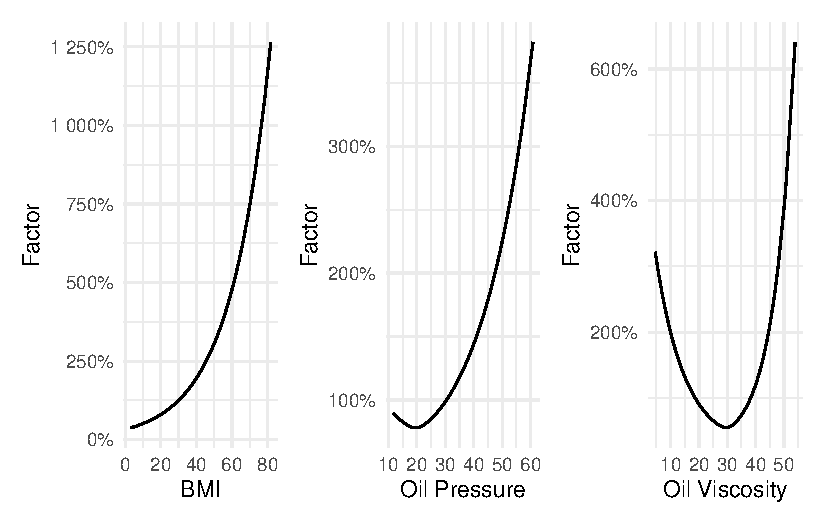
\includegraphics{MakingData_files/figure-pdf/unnamed-chunk-10-1.pdf}

}

\end{figure}

As a result of the increasing mean values of preferred variables, the
distribution of preferred relative risks increases and becomes more
spread out over time.

\begin{Shaded}
\begin{Highlighting}[]
\NormalTok{policy\_pop }\SpecialCharTok{\%\textgreater{}\%}
  \FunctionTok{filter}\NormalTok{(Issue\_Year }\SpecialCharTok{\%in\%} \FunctionTok{c}\NormalTok{(}\DecValTok{2045}\NormalTok{,}\DecValTok{2048}\NormalTok{,}\DecValTok{2051}\NormalTok{,}\DecValTok{2054}\NormalTok{) }\SpecialCharTok{\&}\NormalTok{ PrefFactor }\SpecialCharTok{\textless{}=} \DecValTok{3}\NormalTok{) }\SpecialCharTok{\%\textgreater{}\%}
  \FunctionTok{mutate}\NormalTok{(}\AttributeTok{Issue\_Year=}\FunctionTok{factor}\NormalTok{(Issue\_Year)) }\SpecialCharTok{\%\textgreater{}\%}
  \FunctionTok{ggplot}\NormalTok{(}\FunctionTok{aes}\NormalTok{(}\AttributeTok{x=}\NormalTok{PrefFactor,}\AttributeTok{color=}\NormalTok{Issue\_Year)) }\SpecialCharTok{+}
  \FunctionTok{geom\_density}\NormalTok{(}\AttributeTok{alpha=}\FloatTok{0.2}\NormalTok{) }\SpecialCharTok{+}
  \FunctionTok{scale\_color\_viridis\_d}\NormalTok{(}\AttributeTok{name=}\StringTok{"Issue Year"}\NormalTok{) }\SpecialCharTok{+} 
  \FunctionTok{scale\_x\_continuous}\NormalTok{(}\AttributeTok{name=}\StringTok{"Preferred Relative Risk"}\NormalTok{,}\AttributeTok{labels=}\NormalTok{scales}\SpecialCharTok{::}\NormalTok{percent) }\SpecialCharTok{+}
  \FunctionTok{theme\_minimal}\NormalTok{()}
\end{Highlighting}
\end{Shaded}

\begin{figure}[H]

{\centering 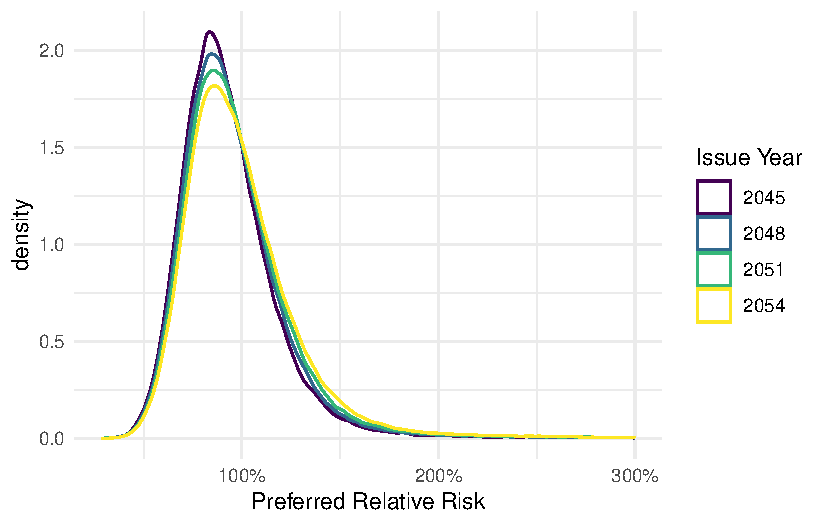
\includegraphics{MakingData_files/figure-pdf/unnamed-chunk-11-1.pdf}

}

\end{figure}

\hypertarget{define-preferred-classes}{%
\subsection{Define Preferred Classes}\label{define-preferred-classes}}

Preferred classes are defined based on old style cutoffs. It is unlikely
that that will still be used in the far future.

\begin{Shaded}
\begin{Highlighting}[]
\NormalTok{policy\_pop[,}
\NormalTok{           UW\_Decision}\SpecialCharTok{:}\ErrorTok{=}\StringTok{"SUB"}\NormalTok{]}
\NormalTok{policy\_pop[BMI }\SpecialCharTok{\textless{}=} \DecValTok{41} \SpecialCharTok{\&}\NormalTok{ OilPressure }\SpecialCharTok{\textless{}=} \DecValTok{41} \SpecialCharTok{\&}\NormalTok{ OilViscosity }\SpecialCharTok{\textless{}=} \DecValTok{32}\NormalTok{,}
\NormalTok{           UW\_Decision}\SpecialCharTok{:}\ErrorTok{=}\StringTok{"STD"}\NormalTok{]}
\NormalTok{policy\_pop[UW\_Decision }\SpecialCharTok{==} \StringTok{"SUB"} \SpecialCharTok{\&}\NormalTok{ PrefFactor }\SpecialCharTok{\textgreater{}} \DecValTok{3}\NormalTok{, }
\NormalTok{           UW\_Decision }\SpecialCharTok{:}\ErrorTok{=} \StringTok{"DEC"}\NormalTok{]}

\NormalTok{policy\_pop[,PrefClass}\SpecialCharTok{:}\ErrorTok{=}\DecValTok{3}\NormalTok{]}
\NormalTok{policy\_pop[BMI }\SpecialCharTok{\textless{}=} \DecValTok{30} \SpecialCharTok{\&}\NormalTok{ OilPressure }\SpecialCharTok{\textless{}=} \DecValTok{35} \SpecialCharTok{\&}\NormalTok{ OilViscosity }\SpecialCharTok{\textless{}=} \DecValTok{25} \SpecialCharTok{\&} 
\NormalTok{             UW\_Decision }\SpecialCharTok{==} \StringTok{"STD"}\NormalTok{,}
\NormalTok{           PrefClass}\SpecialCharTok{:}\ErrorTok{=}\DecValTok{1}\NormalTok{]}

\NormalTok{policy\_pop[BMI }\SpecialCharTok{\textless{}=} \DecValTok{33} \SpecialCharTok{\&}\NormalTok{ OilPressure }\SpecialCharTok{\textless{}=} \DecValTok{38} \SpecialCharTok{\&}\NormalTok{ OilViscosity }\SpecialCharTok{\textless{}=} \DecValTok{28} \SpecialCharTok{\&}\NormalTok{ PrefClass }\SpecialCharTok{\textgreater{}} \DecValTok{1} \SpecialCharTok{\&} 
\NormalTok{             UW\_Decision }\SpecialCharTok{==} \StringTok{"STD"}\NormalTok{,}
\NormalTok{           PrefClass}\SpecialCharTok{:}\ErrorTok{=}\DecValTok{2}\NormalTok{]}
\end{Highlighting}
\end{Shaded}

\hypertarget{simulate-deaths-and-lapses}{%
\subsection{Simulate Deaths and
Lapses}\label{simulate-deaths-and-lapses}}

Simulation relies heavily on multicore computation. Sixteen cores can
get through the mortality simulation for 2,000,000 cases in
approximately 10 minutes. Adjust your expectations accordingly if you
have different resources.

\begin{Shaded}
\begin{Highlighting}[]
\FunctionTok{source}\NormalTok{(}\StringTok{"LoadAssumptions.R"}\NormalTok{)}

\NormalTok{policy\_pop[,}
\NormalTok{           Death\_Duration}\SpecialCharTok{:}\ErrorTok{=}\FunctionTok{mcmapply}\NormalTok{(}\AttributeTok{FUN=}\NormalTok{sample\_death\_duration,}
\NormalTok{                  Sex,}
\NormalTok{                  Issue\_Age,}
\NormalTok{                  Issue\_Date,}
\NormalTok{                  PrefFactor,}
                  \AttributeTok{mc.cores =} \DecValTok{16}\NormalTok{)]}


\NormalTok{policy\_pop[,}
\NormalTok{           Lapse\_Duration}\SpecialCharTok{:}\ErrorTok{=}\FunctionTok{mcmapply}\NormalTok{(}\AttributeTok{FUN=}\NormalTok{sample\_lapse\_duration,}
\NormalTok{                                    Face\_Group,}
                                    \AttributeTok{mc.cores =} \DecValTok{16}\NormalTok{)]}
\end{Highlighting}
\end{Shaded}

\hypertarget{compute-dates-and-status}{%
\subsection{Compute Dates and Status}\label{compute-dates-and-status}}

Deaths do not occur uniformly in a given policy year. As time passes,
risk of death increases. We simulated the policy year of death but not
the day. We do so with a distribution of days tipped toward the later
part of the year. This is designed so that the likelihood of death on
day 365 is about 10\% higher than on day 1.

Lapses occur uniformly through the year on a premium due date. This is
not accurate in the real world, but it is enough for this case study.

\begin{Shaded}
\begin{Highlighting}[]
\NormalTok{death.skew }\OtherTok{\textless{}{-}} \DecValTok{1}\SpecialCharTok{:}\DecValTok{365}
\NormalTok{death.skew }\OtherTok{\textless{}{-}}\NormalTok{ (}\DecValTok{1}\SpecialCharTok{+}\NormalTok{death.skew}\SpecialCharTok{*}\NormalTok{.}\DecValTok{1}\SpecialCharTok{/}\DecValTok{364}\FloatTok{{-}.05{-}.1}\SpecialCharTok{/}\DecValTok{364}\NormalTok{)}\SpecialCharTok{/}\DecValTok{365}

\NormalTok{policy\_pop[,death\_skew\_days}\SpecialCharTok{:}\ErrorTok{=} \FunctionTok{sample.int}\NormalTok{(}\DecValTok{365}\NormalTok{,}
                                         \AttributeTok{size=}\FunctionTok{nrow}\NormalTok{(.SD),}
                                         \AttributeTok{replace=}\NormalTok{T,}
                                         \AttributeTok{prob =}\NormalTok{ death.skew)]}
\NormalTok{policy\_pop[,lapse\_skew\_months }\SpecialCharTok{:}\ErrorTok{=} \FunctionTok{sample.int}\NormalTok{(}\DecValTok{12}\NormalTok{,}\AttributeTok{size=}\FunctionTok{nrow}\NormalTok{(.SD),}\AttributeTok{replace=}\NormalTok{T)]}

\NormalTok{policy\_pop[,}
\NormalTok{           Death\_Date}\SpecialCharTok{:}\ErrorTok{=}\NormalTok{Issue\_Date }\SpecialCharTok{\%m+\%} \FunctionTok{years}\NormalTok{(Death\_Duration}\DecValTok{{-}1}\NormalTok{) }\SpecialCharTok{\%m+\%} 
             \FunctionTok{days}\NormalTok{(death\_skew\_days}\DecValTok{{-}1}\NormalTok{)]}

\NormalTok{policy\_pop[prem\_mode}\SpecialCharTok{==}\StringTok{"M"}\NormalTok{,}
\NormalTok{           Lapse\_Date}\SpecialCharTok{:}\ErrorTok{=}\NormalTok{Issue\_Date }\SpecialCharTok{\%m+\%} \FunctionTok{years}\NormalTok{(Lapse\_Duration}\DecValTok{{-}1}\NormalTok{) }\SpecialCharTok{\%m+\%} 
             \FunctionTok{months}\NormalTok{(lapse\_skew\_months)]}
\NormalTok{policy\_pop[prem\_mode}\SpecialCharTok{==}\StringTok{"A"}\NormalTok{,}
\NormalTok{           Lapse\_Date}\SpecialCharTok{:}\ErrorTok{=}\NormalTok{Issue\_Date }\SpecialCharTok{\%m+\%} \FunctionTok{years}\NormalTok{(Lapse\_Duration}\DecValTok{{-}1}\NormalTok{)]}
\NormalTok{policy\_pop[prem\_mode}\SpecialCharTok{==}\StringTok{"Q"}\NormalTok{,}
\NormalTok{           Lapse\_Date}\SpecialCharTok{:}\ErrorTok{=}\NormalTok{Issue\_Date }\SpecialCharTok{\%m+\%} \FunctionTok{years}\NormalTok{(Lapse\_Duration}\DecValTok{{-}1}\NormalTok{) }\SpecialCharTok{\%m+\%} 
             \FunctionTok{months}\NormalTok{(}\DecValTok{3}\SpecialCharTok{*}\NormalTok{(lapse\_skew\_months }\SpecialCharTok{\%\%} \DecValTok{4} \SpecialCharTok{+} \DecValTok{1}\NormalTok{ ) )]}

\NormalTok{policy\_pop[,Status}\SpecialCharTok{:}\ErrorTok{=}\StringTok{"Active"}\NormalTok{]}
\NormalTok{policy\_pop[Death\_Date }\SpecialCharTok{\textless{}=} \FunctionTok{ymd}\NormalTok{(}\DecValTok{20531231}\NormalTok{) }\SpecialCharTok{\&}\NormalTok{ Death\_Date }\SpecialCharTok{\textless{}}\NormalTok{ Lapse\_Date,}
           \StringTok{\textasciigrave{}}\AttributeTok{:=}\StringTok{\textasciigrave{}}\NormalTok{(}\AttributeTok{Status=}\StringTok{"Death"}\NormalTok{,}\AttributeTok{Term\_Date=}\NormalTok{Death\_Date)]}
\NormalTok{policy\_pop[Lapse\_Date }\SpecialCharTok{\textless{}=} \FunctionTok{ymd}\NormalTok{(}\DecValTok{20531231}\NormalTok{) }\SpecialCharTok{\&}\NormalTok{ Lapse\_Date }\SpecialCharTok{\textless{}}\NormalTok{ Death\_Date,}
           \StringTok{\textasciigrave{}}\AttributeTok{:=}\StringTok{\textasciigrave{}}\NormalTok{(}\AttributeTok{Status=}\StringTok{"Lapsed"}\NormalTok{,}\AttributeTok{Term\_Date=}\NormalTok{Lapse\_Date)]}

\NormalTok{policy\_pop[UW\_Decision}\SpecialCharTok{==}\StringTok{"DEC"}\NormalTok{,}
           \StringTok{\textasciigrave{}}\AttributeTok{:=}\StringTok{\textasciigrave{}}\NormalTok{(}
             \AttributeTok{Status=}\StringTok{"Not Issued"}\NormalTok{,}
             \AttributeTok{Term\_Date=}\ConstantTok{NA}
\NormalTok{           )]}
\end{Highlighting}
\end{Shaded}

\hypertarget{save-the-work}{%
\subsection{Save the Work}\label{save-the-work}}

\begin{Shaded}
\begin{Highlighting}[]
\NormalTok{arrow}\SpecialCharTok{::}\FunctionTok{write\_parquet}\NormalTok{(}\AttributeTok{x=}\NormalTok{policy\_pop,}
                     \AttributeTok{sink=}\StringTok{"policy\_pop.parquet"}\NormalTok{)}
\end{Highlighting}
\end{Shaded}




\end{document}
